\chapter{Systeme}
\label{cha:systeme}

\section{Samsung Knox}


Ist man Besitzer aktueller Samsung-Geräten findet man die Applikation \textit{Sicherer Ordner}\footnote{Sicherer Ordner löste am 19. Dezember 2017 den Vorgänger MyKnox ab {sam2017b} }als vorinstallierte Standardsoftware vor. Mit Öffnen dieser App können, nach Eingabe eines benutzerdefinierten Sicherheitsverfahren, verschiedene Einstellungen getätigt werden. Es ist möglich Dateien oder Apps in diesen ""sicheren Ordner" zu verschieben. Sogar Apps die vorher nicht auf dem Smartphone vorhanden sind, können direkt vom Store geladen und installiert werden.Theoretisch wäre dieser Lösungsansatz genau richtig für die Verwendung von BYOD und zusätzlich sogar kostenlos. Dennoch wäre dies nicht umsetzbar im Enterprise-Umfeld.

Um den Anforderungen an eine BYOD-Lösung der Loco AG gerecht zu werden, benötigt es eine MDM-Möglichkeit. Dafür muss die IT-Administration die Möglichkeit haben die eingesetzten Geräte zu verwalten und somit an die firmeninternen Sicherheitsanforderungen anzupassen. Eine mögliche Lösung bietet Samsung mit der kostenpflichtigen Variante Samsung Knox Premium, die im Folgenden nach dem Kriterienkatalog belichtet werden soll.


Das Sicherheitsverfahren der Knox-Plattform aus fünf Komponenten \cite{sam2017}:
\begin{enumerate}
\item Mehrschichtige Sicherheit
\item Root-of-Trust
\item Secure Boot und Trusted Boot
\item TrustZone®
\item SE for Android
\end{enumerate}




\section{MobileIron}

\subsection {Allgemein} 
Das Unternehmen MobileIron ist ein US-amerikanisches Unternehmen mit Hauptsitz in Kalifornien welches im Jahr 2007 gegründet wurde. MobileIron hat sich von Anfang an auf die Verwaltung von mobilen Endgeräten im Enterprise Umfeld spezialisiert. Das Unternhemen wurde 2017 im siebten Jahr in folge als Leader im Magic Quadrant von der Gartner Inc. neben VMWare, IBM und BlackBerry für MDM/EMM Suites gekürt. Das Softwareentwicklungsunternehmen bietet in Ihrem Produktportfolio verschiedene Bring Your Own Device Pakete mit zahlreichen Funktionen an. 
\subsection {Kompatibilität}
\subsection {Paketmodelle}
MobileIron bietet die drei verschiedenen Bundles „EMM Silver“, „EMM Gold“ oder „EMM Platinum“ seiner Bring Your Own Device Lösung an.
Das Basispaket „EMM Silver“ beinhaltet die Komponenten „Core“ „Sentry „und „Apps@Work“. Das Paket „EMM Gold“ ist um die Module „Email+“, „Docs@Work“ und „Web@Work“ erweitert. Durch die Wahl des Platinum Pakets ergänzt sich dieses wiederum um „Help@Work“, „Tunnel“, „MobileIron Monitor“ und „ServiceConnect-Integration“.

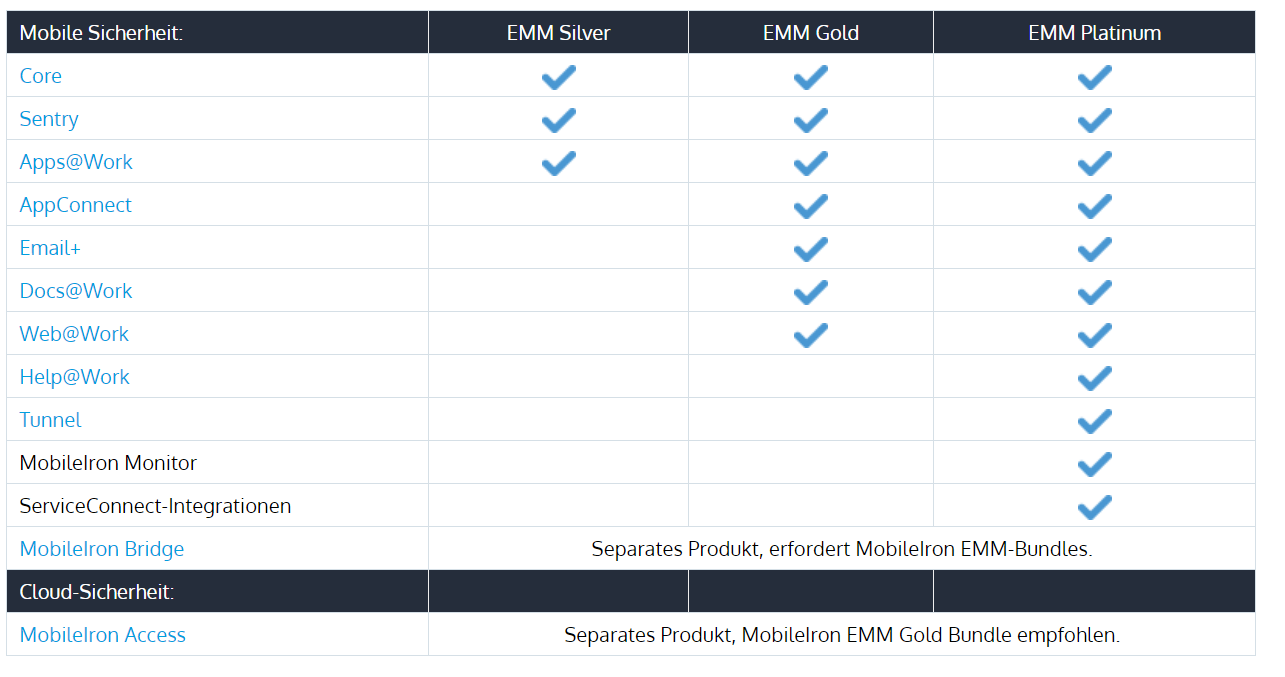
\includegraphics[width=0.95\textwidth]{Bilder/mi_1.png} 

\subsection {Pakete}
\subsubsection {Core}
Das Paket Core ist das zentrale Modul, welches das IT-Backend des Unternhemens einbindet. Hierüber können die erforderlichen Sicherheits- und Verwaltungsrichtlinen der mobilen Endgeräte definiert und verwaltet werden. Über die  API Schnittstellen des Cores kann man komfortabel Erweiterungen nurzen. Im Fokus des Cores stehen jedoch die das MDM, MAM und MCM. Der Core bietet für die Administratoren zusätzliche Analyse- und Auswerungsfunktionen. So kann beispielsweise der von den Endgeräten produzierten Netzwerktraffic ausgewertet werden um Infrastrukturprobleme zu lokaliseren. Durch die Möglichkeit Dashboards-Widgets anzulegen kann der Administrator das System und die verschiedenen Gerätestatuus komfortabel überblicken. 
\subsubsection {Sentry}
Die Komponente Sentry ist das Inline-Gateway, das den gesamten Netzwerkverkehr zwischen den Mobilgeräten und dem Unternehmensbackend verschlüsselt, verwaltet und sichert. Sentry setzt die in der Core Komponente definierten Sicherheitsrichtlinien um. Sentry kann beispielsweise E-Mail Anhänge verschlüsseln, sodass nicht authorisierte Applikationen auf diese Daten nicht zugreifen können. 

\subsubsection {Apps@Work}
Apps@Work ist ein unternhemenseigener App Store, indem sowohl eigenentwickelte als auch öffentliche, freigegebene Anwendungen für die Benutzer bereitgestellt werden können. Über diesen Weg können Administratoren schnell auswählen, welche Anwendungen erforderlich, zulässig oder verboten sind. 
\subsubsection {AppConnect}
\subsubsection {Email+}
\subsubsection {Docs@Work}
\subsubsection {Web@Work}
\subsubsection {Help@Work}
\subsubsection {Tunnel}
\subsubsection {MobileIron Monitor}
\subsubsection {ServiceConnect-Integration}

Das ist der Core

\subsection {Abrechnungsmodell}

Je nach Tarifplänen bzw. Paketangeboten werden neben den genannten Grundfunktionen weitere Features unterstützt. Das Unternehmen selbst betreibt ein sehr flexibles Abrechnungsmodell, welches auf jegliche Bedürfnisse des Endkunden angepasst werden kann. Dabei kann beispielsweise zwischen einer Lizenzierung pro Benutzer (maximal 3 Endgeräte) oder einem Lizenzierungsmodell je nach Endgerät gewählt werden. Neben der Kaufoption von Lizenzen auf Lebenszeit wird auch ein Abonnement angeboten. Neben der klassischen Installation innerhlab des eigenen Netzwerks betreibt MobileIron auch eine eigene Cloud die für die Bereitstellung der Services genutzt werden kann. Falls sich der Endkunde für die Cloudlösung entscheidet kann direkt ein erweiterter Support (SLA) dazugebucht werden. Für die Installation auf einem eigenen System kann hierbei nur zwischen einem Standard- und Premiumsupport unterschieden werden.  

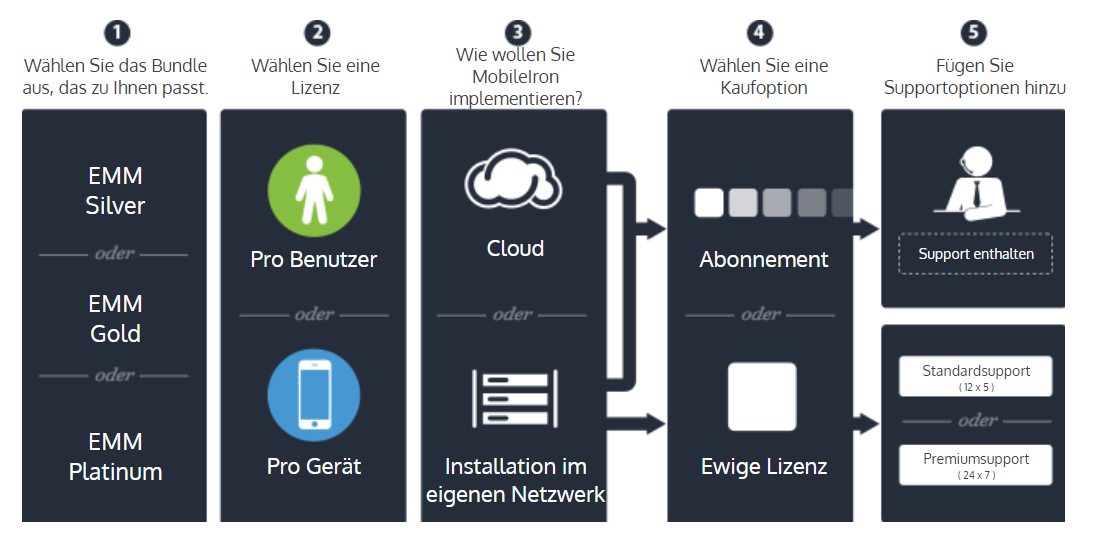
\includegraphics[width=0.95\textwidth]{Bilder/mi_2.png} 